% !TeX encoding = UTF-8
% !TeX spellcheck = en_US
% !TeX root = ../MasterThesis_OlivierChurlaud_2016.tex
\tikzset{
	block/.style = {draw, fill=white, rectangle, minimum height=3em, minimum width=4em},
	gain/.style = {draw, fill=white, isosceles triangle, minimum height=3em, minimum width=2em},
	operator/.style= {draw, fill=white, circle},
	input/.style = {coordinate},
	output/.style= {coordinate},
	pinstyle/.style = {pin edge={to-,thin,black}},
}

\chapter{Orbit correction}
\label{sec:correction}

\section{Motivation}
The accelerators are designed so that the particles follow a given path, which is defined in the case of synchrotrons by the successive bending involved by dipole magnets. Quadrupole magnets are additionally needed to provide focusing and guarantee the closing of the orbit. As the precision of the positioning of the magnets is limited, some errors may destabilize the orbit and increase the deviation of the particles around the theoretical orbit.

In addition, the environment produces perturbations: for instance the 50~Hz of the main power, some not perfectly isolated magnetic sources (like the booster at \SI{10}{\hertz}). \Cref{fig:fft_no_correction} shows the spectrum of the beam displacement from the reference orbit before correction. 
\begin{figure}
	\centering
	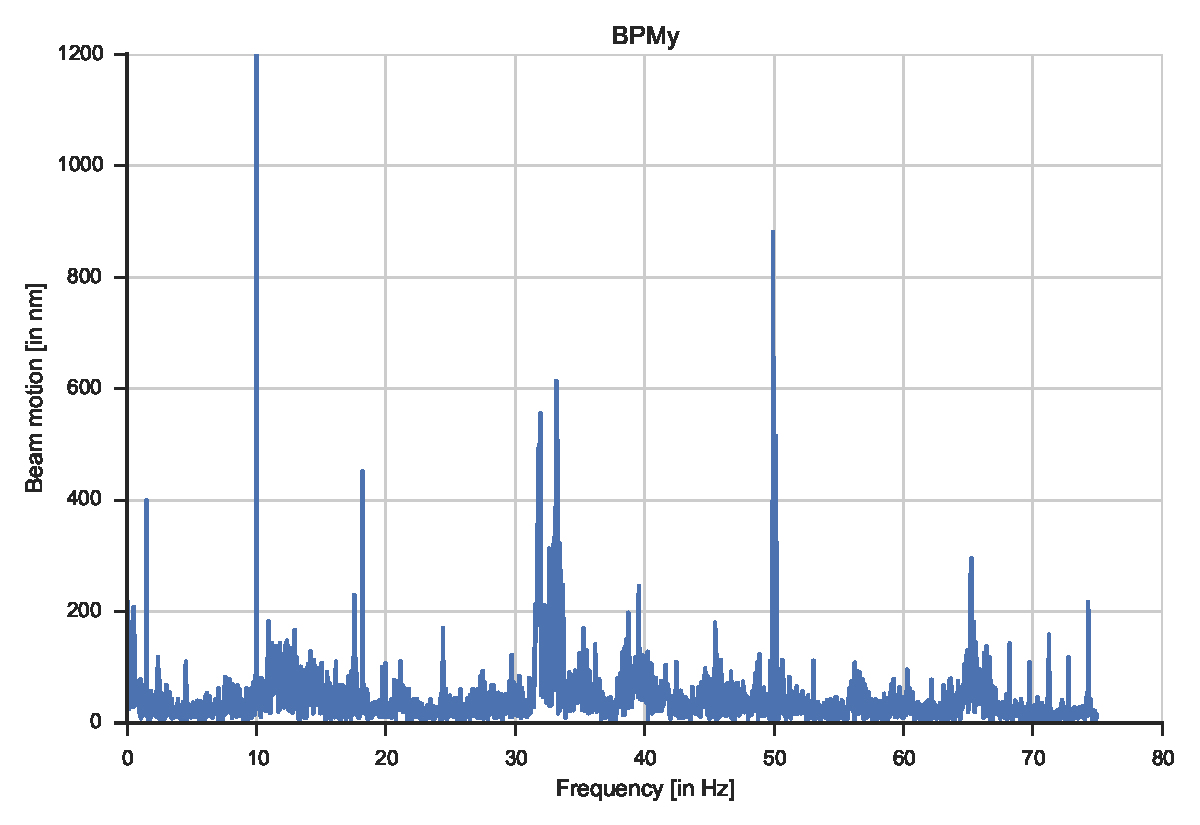
\includegraphics[width=.9\linewidth]{img/fft_no_corr}
	\caption{\label{fig:fft_no_correction} Spectrum of the beam motion, without correction (vertical)}
\end{figure}

In order not to lose electrons in the walls of the vacuum chamber but also to increase the brightness of the synchrotron radiations (and therefore to have focused electron beams), all these residual misalignment and magnetic field errors must be corrected.

The most classical correction methods will be presented here, before explicitly describing the case of BESSY~II and the ameliorations proposed during this thesis.

\section{Monitoring and correction instruments}
To be able to correct the orbit or localize perturbations, some tools must be employed.

\subsection{Beam Position Monitors}
The position of the beam in a given direction is monitored with beam position monitors (BPM).

Several types of BPMs exist, but the important characteristics of the one used at BESSY~II are that they provide a method
\begin{itemize}
	\item which is non invasive (it does not affect the beam or negligibly)
	\item which outputs an electric signal proportional to the distance of the beam from an arbitrary point.
\end{itemize}

This last property means that the measured value must always be subtracted by a reference value.

The raw values output by the BPMs are thus never considered and every orbit position value given (also called BPM value by misuse of language) is always, at position~$s$ and time~$t$
\begin{equation}
\Delta x_\text{BPM}(s,t) = x_\text{BPM}(s,t) - x_\text{BPM,ref}(s)
\end{equation}

\subsection{Correctors}
To correct the orbit, BESSY~II uses dipole magnets, also called corrector magnets (CM) positioned around the storage ring. Each dipole contributes to correcting in a given direction, at a specific position.

\subsection{Monitor and corrector numbers}
The number of monitors and correctors is quite important. Because the correction method used is based on an inversion problem (see \cref{sec:response_matrix}), it is important to have an over-constrained problem. Else a perfect correction would be reached at monitor positions but unconstrained (and thus potentially arbitrary bad) elsewhere.

Therefore the number of BPMs is chosen quite greater than the number correctors.

At BESSY~II there are
\begin{itemize}
	\item 128~BPMs, measuring both horizontal ($\text{BPM}_\text{x}$) and vertical ($\text{BPM}_\text{y}$) direction,
	\item 48~CMs for the horizontal direction ($\text{CM}_\text{x}$) and 64 for the vertical one ($\text{CM}_\text{y}$).
\end{itemize}

\section{Some documented methods}
Several global corrections methods are well documented in the literature. Local orbit bumps (presented in \cref{sec:orbit_bump}) allow local correction and are used to change the path of the orbit (during the injection time for example). The most common ones are the best corrector method and the response matrix method (see \cref{sec:most_effective_corr,sec:response_matrix}), as they provide a global correction, over the whole orbit.

\subsection{Local orbit bumps}
\label{sec:orbit_bump}
Using local orbit bumps is a basic method that gives total control on the orbit local modification to the operator.

\subsubsection{Principle}
Adding a simple dipole on the path of a particle will bring it closer or push it away. As the particles must eventually return to the planned orbit, a series of dipoles can be set one after the other to design an arbitrary path. \Cref{fig:local_bump} shows a minimal example, where the black points represent the magnets, and the dashed line the original orbit. Each magnet $M_i$ has position $s_i$, where the phase is $\Psi_i$ and the beta function  $\beta_i$. The orbit motion at this position is described by the vector $\vec{x}_i = (x_i , x'_i)$.
\begin{figure}
	\centering
	\begin{tikzpicture}[auto, node distance=1.2,>=latex']
	%\draw[help lines, yellow] (-1,-4)grid(15,3);
	% We start by placing the blocks
	\coordinate [] (lleft) {};
    \coordinate [right=.2 of lleft] (origin) {};
    \coordinate [below=.2  of origin] (xaxisbottom) {};
    \coordinate [above=2 of origin] (xaxistop) {};
	\node [draw, circle, fill=black, right=2 of lleft, label=below:$M_1$] (leftm) {};
    \node [draw, circle, fill=black, right=3 of leftm, label=below:$M_2$] (middlem) {};
	\coordinate [above=1.5 of middlem] (topcoord) {};
	\node [draw, circle, fill=black, right=4 of middlem, label=below:$M_3$] (rightm) {};
	\coordinate [right=2 of rightm] (rright) {};
	% Once the nodes are placed, connecting them is easy.
	\draw [-] (lleft) -- (leftm);
	\draw [-] (leftm) to [bend left=35] (topcoord);
	\draw [-] (topcoord) to [bend left=35] (rightm);
	\draw [->] (rightm) -- node [near end] {$s$} (rright);
    \draw [->] (xaxisbottom)  -- node [near end]{$x$} (xaxistop);
   	\draw [dashed] (leftm) -- (rightm);
	\end{tikzpicture}
	\caption{\label{fig:local_bump}Local bump with 3 magnets (inspired by~\cite{book:wille}, Fig~3.47)}
\end{figure}

The strengths $\kappa_1$, $\kappa_2$, $\kappa_3$ of each magnets can be calculated with the formalism introduced in \cref{sec:beta_func}, \cref{eq:motion_transfert_matrix} in order to achieve the right displacement and respect the closed orbit condition. The following conditions must be fulfilled (closed orbit):
\begin{equation}
\vec{x}_1 = \dbinom{0}{\kappa_1} \qquad \text{and} \qquad
\vec{x}_3 = \dbinom{0}{-\kappa_3}
\end{equation}

The orbit motion at $s_3$ is the superposition of the effects of $M_1$ and $M_2$ alone. It can thus be written
\begin{equation}
\vec{x}_3 = \mat{M}_{1 \rightarrow 3} \vec{x}_1 + \mat{M}_{2 \rightarrow 3} \dbinom{0}{\kappa_2}
\end{equation}
or
\begin{equation*}
\begin{pmatrix} 0 \\ -\kappa_3 \end{pmatrix} =
\begin{pmatrix} a_{11} & a_{12} \\ a_{21} & a_{22} \end{pmatrix} \begin{pmatrix} 0 \\ \kappa_1 \end{pmatrix} +
\begin{pmatrix} b_{11} & b_{12} \\ b_{21} & b_{22} \end{pmatrix} \begin{pmatrix} 0 \\ \kappa_2 \end{pmatrix}
\end{equation*}
Solving this system of equations and replacing the coefficients of the matrix by their expression in \cref{eq:motion_transfert_matrix} leads to the values of $\kappa_2$ and $\kappa_3$ in function of $\kappa_1$ (see \cite{book:wille}, p.130 for the exact equations). This can allow an arbitrary displacement of the orbit at a given position. This can be extended to a version with $N$ magnets, which allows the free setting of $N-2$ parameters ($x$ or $x'$). This is extensively described in \cite{book:wille}.

\subsubsection{In practice}
This solution is used for instance to shift a part of the orbit during particle injections, in order not to disturb already stored particles. It can also be used to counter a known localized perturbation which source cannot be removed.

It is indeed very efficient to locally shift the orbit. However it cannot be used for correction, as it needs a precise knowledge of the optic of the ring, which is not the case (some devices have no theoretical optic model). Further more, it would be an iterative method as the correction would need to be calculated and applied for each orbit segment.

\subsection{Most effective corrector method}
\label{sec:most_effective_corr}
This method is based on the fact that orbit shifts are often caused by strong localized disturbances. Its goal is to correct particularly each disturbance.

\subsubsection{Principle}
Given a distorted orbit, the optimal gain for each corrector is calculated by a mean square error algorithm (see \cref{eq:gain_bestcorr} and \cite{book:wille}). The corrector which provides the best correction is selected: it is the most effective corrector.

Let's assume that the $i$th corrector, at position $s_i$, has the optical parameters $\beta_i$, $\alpha_i$ and $\Psi_i$, and that $m$ monitors are set around the orbit with parameters $\beta_j$, $\alpha_j$ and $\Psi_j$, and read a displacement $u_j$ from the reference orbit ($1 \leq j \leq m$).

The strength $\kappa_i$ of the field at the position $s_i$ is obtained minimizing the function
\begin{equation}
	\label{eq:gain_bestcorr}
    f_i(\kappa_i) = \sum\limits_{j=1}^{m} (u_j-x_{ij}(\kappa_i))^2
                  = \sum\limits_{j=1}^{m} (u_j- \kappa_i h_{ij})^2
\end{equation}

with, if $\Delta \Psi_{ij} := \Psi_j-\Psi_i$,

\begin{align}
    \label{eq:hij}
    x_{ij}(\kappa_i) &= \kappa_i h_{ij} \nonumber\\
                     &= \kappa_i \frac{\sqrt{\beta_i \beta_j}}{2}
                         \left[
                             \frac{\cos(\Delta \Psi_{ij}) - 2\alpha_i \sin(\Delta\Psi_{ij})}
                                  {\tan (\pi Q)} + \sin (\Delta\Psi_{ij})
                         \right].
\end{align}

It follows that
\begin{equation}
    \kappa_i = \frac{\sum\limits_{j=1}^m u_j h_{ij}}{\sum\limits_{j=1}^m h_{ij}^2}
\end{equation}

The $i$th corrector is attributed the gain $-\kappa_i$ to compensate the field.

\subsubsection{Iterative version}
When the most effective corrector is found, the process is reiterated on the corrected orbit with the remaining correctors. By doing this until all corrector are used (or that adding a correction does not improve the orbit) a comprehensive correction is reached.

\subsubsection{Practical issue}
The problem of this method is that each corrector must be tested once, and this for each iteration: the initialization of the correction is long and is then fixed. Moreover, the correction is less efficient than the other ones presented here~\cite{book:wille}.

\subsection{Response matrix}
\label{sec:response_matrix}
This section is mainly based on~\cite{book:wille}, \cite{art:decker-1991} and \cite{art:plouviez-1999}.

\subsubsection{Inverse problem}
This correction is based on solving the following inverse problem: the expected orbit being known, how to set the correctors in order to achieve it? To solve it, the response matrix $\mat{S}$ is introduced.

The response matrix $\mat{S}$ is defined by the equation $\vec{X} = \mat{S}\, \vec{\Theta}$ where $\vec{\Theta}$ is the \emph{kick vector} (i.e. the vector of strength of the field generated by each corrector) and $\vec{X}$ the vector of \emph{orbit change}. If the accelerator has $M$ monitors and $N$ correctors, then $\mat{S}$ is a $M \times N$ matrix. $\mat{S}$ is often termed \emph{forward} or \emph{observation matrix} because it describes the effects of a given phenomenon. Indeed, each coefficient $S_{ij}$ of the matrix is the orbit change at the position $s_i$ (of the $i$th monitor), for a kick of unity 1 at the position $s_j$ (of the $j$th corrector).

Inversing the response matrix will provide the correction to apply. Since it's very common to have more monitors than correctors, the matrix is not square. A \emph{singular value decomposition} (SVD) is used on the matrix to provide a pseudo-inversion $\mat{S}^*$ of $\mat{S}$.

Using the SVD also allows to use only the most significant singular values in the correction. This prevents to over-correct the orbit, by not considering less significant values that can result of noise in the monitors during the measure, numerical artifacts or incorrections in the response matrix.

The correction can then be performed
\begin{equation}
\vec{\Theta} = \mat{S}^* \vec{X}.
\end{equation}

\subsubsection{Acquisition of the response matrix}
Before solving the inverse problem, the response matrix must first be determined. This can be achieved in two different ways: by describing the magnet structure and explicitly calculating the matrix or by acquiring it in an experimental way.

\paragraph{Calculation of the response matrix}
The matrix can be theoretically calculated by using the accelerator model and physics. This was already used in \cref{sec:most_effective_corr} and using the same calculations leads to setting, for the $i$th monitor and $j$th corrector,
\begin{equation}
S_{ij} = h_{ij}
\end{equation}
with $h_{ij}$ as defined in \cref{eq:hij}.

The main flaw of this method is that it is only a model which hence may not exactly represent the reality. Some misalignments of magnets or external magnetic perturbations would not be taken in account. It's however a good first approach.

\paragraph{Experimental acquisition of the response matrix}
A more common and precise way of constructing the response matrix is empirical: it suffices to give a unitary value to a corrector and to read the monitors to obtain a column $\mat{S}$. Doing so for each corrector provides the whole matrix.


\section{State of the art at BESSY II}
\label{sec:correction_state_of_art}
BESSY II currently implements a Fast Orbit Feedback (FOFB) which is based on the response matrix inverse. The correction algorithm will be first described in \cref{sec:correction_sa_corr}, and current choices will be discussed by references found in literature. A technical overview will then be provided in \cref{sec:correction_sa_technical}, presenting the actual processes taking part in the correction.

\subsection{The correction}
\label{sec:correction_sa_corr}
Using the response matrix to correct the orbit is quite common \cite{book:wille,art:plouviez-1999,art:li-2001}. However, as already highlighted in \cref{sec:response_matrix}, the matrix never perfectly represents the orbit and because of noises in the environment, it is not sufficient. In general only the largest singular values are used and some corrections are additionally needed in the frequency domain.

To cope with these additional requirements, a PID correction (proportional response with gain $K_p$, integral response with gain $K_i$ and derivative response with gain $K_d$) is used at BESSY~II. It also deals with the delays introduced by the process between the time the orbit is read by the BPMs and the moment the correction is actually applied \cite{art:plouviez-1999}.

The full process goes as presented in \cref{fig:block_correction}.

\begin{figure}
    \centering
    \begin{tikzpicture}[auto, node distance=1.2,>=latex']
    %\draw[help lines, yellow] (-1,-4)grid(15,3);
        % We start by placing the blocks
        \node [operator] (sum) {$+$};
        \node [input, above=2 of sum.center] (xref) {};
        \node [operator, right=of sum] (prod) {$\times$};
        \node [input, above=2 of prod.center] (invS) {};
        \node [gain, right=0.7 of prod] (gain) {$\vec{W}$};
        \node [block, right=of gain] (PID) {~PID~~};
        \node [input, above=2 of PID.center] (pidcoef) {};
        \node [operator, right= of PID] (sum2) {$+$};
        \node [block, above right= 0.8 and 0.65 of sum2.center] (delay) {Delay T};
        \coordinate [right=3 of sum2.center] (straight) {};
        \node [draw, ellipse, minimum height=1.7cm, minimum width=5.5cm, below=1 of straight] (ring) {Storage Ring};
        \node [draw, ellipse, line width=1pt, dotted, minimum height=.5cm, minimum width=.8cm, above=-.25 of ring.north, label=above right:\footnotesize Correctors] () {};
        \node [draw, ellipse, line width=1pt, dotted, minimum height=.5cm, minimum width=.8cm, above=-.25 of ring.west, label=above left:\footnotesize BPMs] (BPM) {};
        \coordinate [left=1 of sum.center](leftback) {};

        % Once the nodes are placed, connecting them is easy.
        \draw [->] (xref)     -- node [pos=0.85, left]{$-$} node {$\vec{X}_\text{ref}$}(sum);
        \draw [->] (sum)      -- node {$\Delta\vec{X}$} (prod);
        \draw [->] (invS)     -- node {$\mat{S}^*$}        (prod);
        \draw [->] (prod)     -- node {}             (gain);
        \draw [->] (gain)     -- node {$\Delta\vec{\Theta}_\text{t}$}             (PID);
        \draw [->] (PID)      -- node {$\Delta\vec{\Theta}$} node[pos=0.80, below] {$-$}      (sum2);
        \draw [->] (pidcoef)  -- node[pos=0.70, above, fill=white] {PID coeff.} (PID);
        \draw [-]  (sum2)     -- node {}  (straight);
        \draw [->] (straight) |- node[pos=0, right] {$\vec{\Theta}_{(n)}$} (delay);
        \draw [->] (delay)    -| node[above] {$\vec{\Theta}_{(n-1)}$} (sum2);
        \draw [->] (straight) -- node[pos=0.80] {}  (ring);
        \draw [-]  (ring)     -| node {}             (leftback);
        \draw [->] (leftback) |- node[pos=0.5] {$\vec{X} $}  (sum.west);
\end{tikzpicture}
    \caption{\label{fig:block_correction}The correction process used at BESSY~II}
\end{figure}

The control value at correction cycle $n$ is the differential orbit
\begin{equation}
 \Delta \vec{X}[n] := \vec{X}[n]-\vec{X}_\text{ref}
\end{equation}
which is expected to be close to 0. The correction provided by the weighted response matrix is then processed
\begin{equation}
\Delta \vec{\Theta}_\text{t}[n] :=  \left(\mat{S}^{-1} \cdot \Delta \vec{X}[n] \right) \odot \vec{W}
\end{equation}
(with $\odot$ the point-wise multiplication and $\vec{W}$ the vector of weights) and modulated by the PID correction. The ideal PID in the Laplace form is described with
\begin{equation}
H_{PID}(s) = K_p + \frac{K_i}{s} + K_d \cdot s
\end{equation}
or, with the z transform (calculated with Euler's method),
\begin{equation}
H_{PID}(z) = K_p + \frac{K_i}{1-z} + K_d \cdot (1-z)
\end{equation}
which yields
\begin{equation}
\Delta \vec{\Theta}[n] =  K_p \cdot \Delta \vec{\Theta}_\text{t}[n] + K_i \cdot \sum\limits_{k=0}^{n-1}\Delta \vec{\Theta}_\text{t}[k] + K_d \cdot \left(\Delta \vec{\Theta}_\text{t}[n] - \Delta \vec{\Theta}_\text{t}[n-1]\right).
\end{equation}

The real correction is eventually the accumulation of all corrections
\begin{equation}
\vec{\Theta}(n) = \vec{\Theta}[n-1] - \Delta \vec{\Theta}[n].
\end{equation}

For stability reasons, the PID was always implemented as a pure proportional corrector ($K_i$ and $K_d$ being set to zero). Indeed, because of the last accumulation, it was of course behaving like a proportional integrator (PI), which forbade the use of the other coefficients in the PID correction. In the simulations described in \cref{sec:correction_simulation}, a corrector PID can be implemented with more optimal coefficients. It is however important that the correction starts from an initial value known to be stable, so that the beam stays focused.

\subsection{Technical overview}
\label{sec:correction_sa_technical}
The correction is naturally automatized. Because the read/write actions should be really fast, a specific infrastructure was designed. This is represented on \cref{fig:cbox_mbox}.

\begin{figure}[!h]
    \centering
    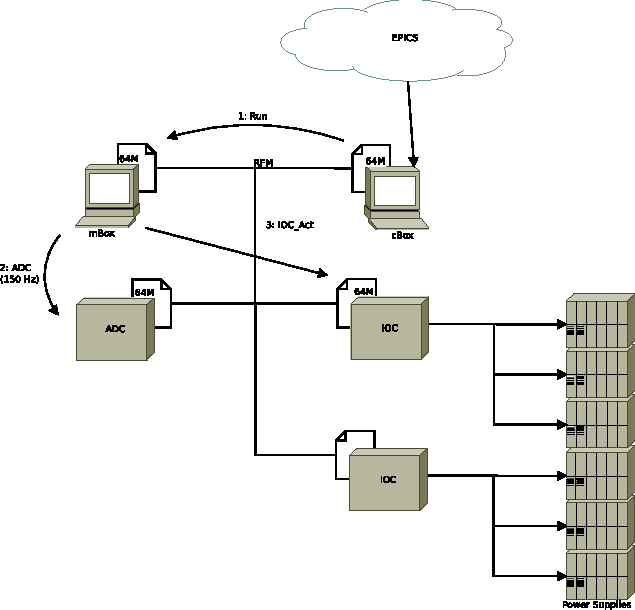
\includegraphics[width=.85\linewidth]{img/mBox_cBox}
    \caption{\label{fig:cbox_mbox}cBox and mBox: the correction infrastructure at BESSY~II}
\end{figure}

All elements are connected to a reflective memory (RFM), which provides a high speed and low latency interface. This memory space is split in specified divisions to prevent data collisions: one part contains the configuration, a second the orbit values and the last one the correction values.

\paragraph{Actors}
The following actors are playing a role in the process:
\begin{itemize}
    \item the \textbf{analog-to-digital converter (ADC)} reads the orbit displacement values from the BPMs and makes them available to the other actors.
    \item the \textbf{cBox} controls (= \textit{c}) the correction. It defines when to read the values of the BPMs and when to write the new correction values, it provides initializations values. The operators are communicating with this process to configure the correction.
    \item the \textbf{mBox} does the math (= \textit{m}) of the correction. When allowed by the cBox, it reads the BPMs values, do the maths to define the new correction values (multiplication with the response matrix, PID correction) and write them to the communication bus. This process also publish the values it reads and writes so that client programs can subscribe to this data stream and reuse the values internally.
    \item the \textbf{input-output controllers (IOCs)} write the correction values to the power supplies commands when they are available.
    \item the \textbf{power supplies (PS)} provide a given power to the corrector magnets.
\end{itemize}

\paragraph{Process description}
After having received the authorization to run from the cBox, the mBox process starts. It first does its full initialization, which only happens on start (the response matrix, the reference orbit, the PID parameters, etc. cannot change while the mBox process is running), and starts the ADC. From this time, the ADC will write new orbit values to the RFM at a rate of \SI{150}{\hertz}.

The mBox waits for the ADC interruption to read the new orbit data from the RFM. The correction is then calculated (in Amperes) and the values are converted in the DAC input format (basically unsigned integers). This data is written back to RFM and an interruption is sent to inform the other elements that the new values are available. This is read by the IOCs that relay to the power supplies alimenting the corrector magnets.

This defines a real time process, repeated at the frequency of \SI{150}{\hertz}.

The duration of each step is as following:
\begin{itemize}
\item orbit value acquisition (BPMs): 0.3 to \SI{1.7}{\milli\second}
\item correction computation: 0.5 to \SI{1}{\milli\second}
\item transmission of the correction date to the power supplies: 0.5 to \SI{1}{\milli\second}
\end{itemize}

\remark One of the side works done during this thesis was rewriting the whole mBox in C++ in a very object oriented way to allow a smaller computation time (the original one was written in \textsc{Matlab}), easier improvement and feature additions (like a dynamic correction, easier communication with external scripts, production/experimental modes, etc.). This is fully presented in \cref{apx:mbox}.

\subsection{Result overview}
The results of this correction can be seen on \cref{fig:compare_fofb}: the low frequencies and most of the peaks are reduced, which is a real gain for the end users of the accelerator. Unfortunately, the correction gain provides only a correction up to $\sim\!\SI{12}{\hertz}$., and increasing it let the system become instable. Such a correction is therefore not always sufficient and other methods are experimented to decrease the remaining disturbances.

\begin{figure}
    \centering
    \begin{subfigure}[b]{0.8\textwidth}
        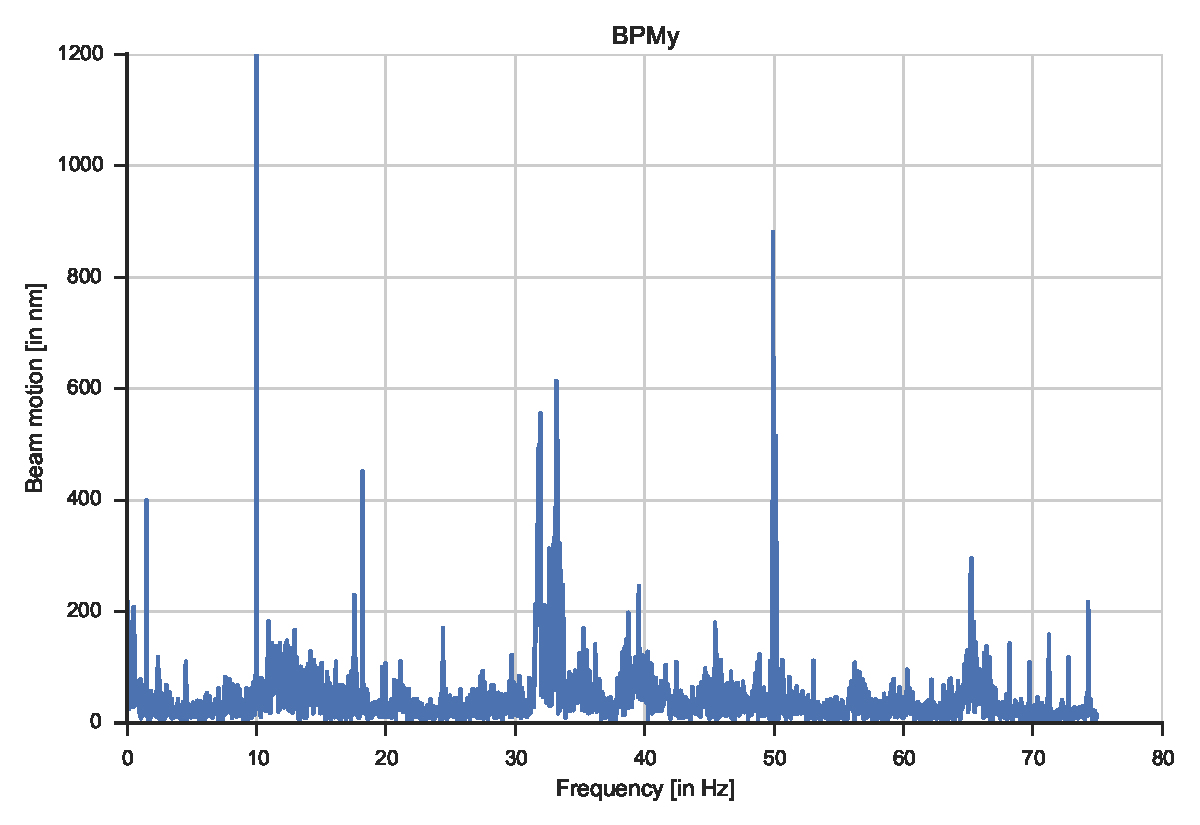
\includegraphics[width=\linewidth]{img/fft_no_corr}
        \caption{No correction}
    \end{subfigure}
    
    \begin{subfigure}[b]{0.8\textwidth}
        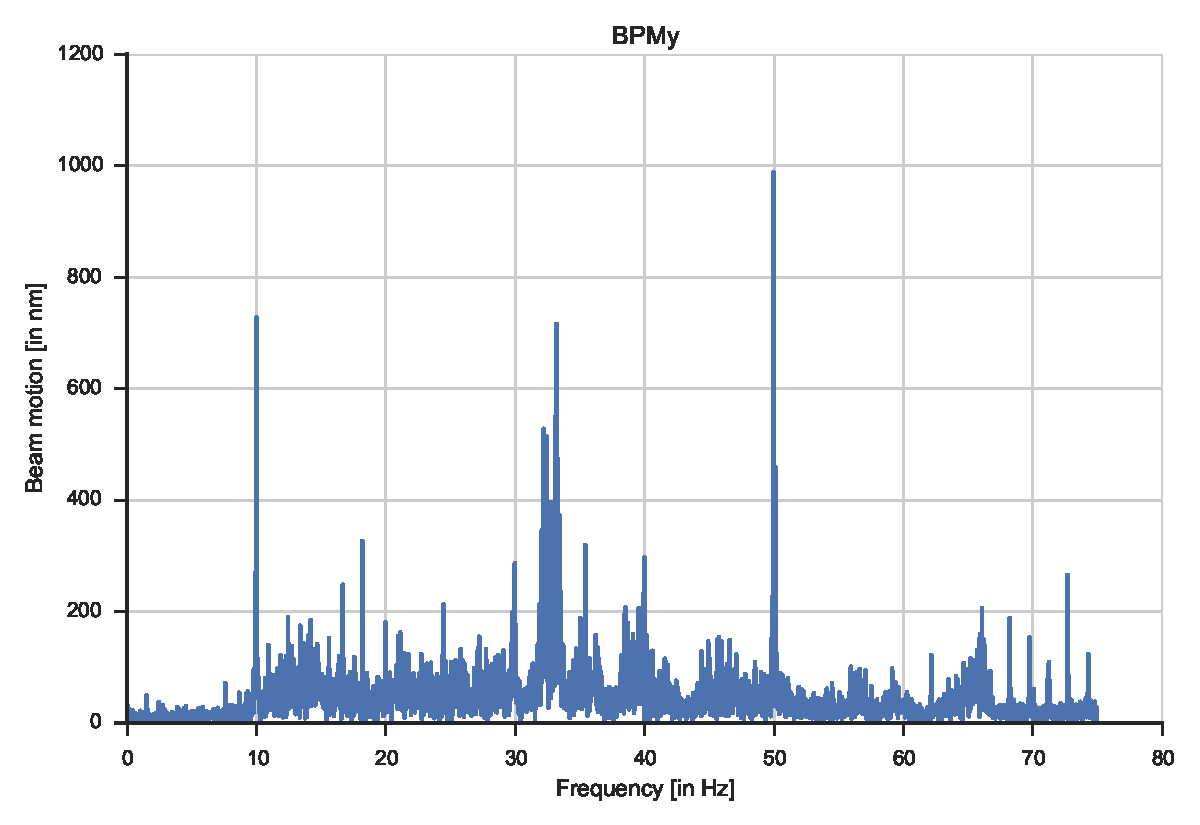
\includegraphics[width=\linewidth]{img/fft_fofb}
        \caption{FOFB correction}
    \end{subfigure}
    \caption{\label{fig:compare_fofb}Orbit motion spectrum: with and without FOFB (vertical, current: \SI{300}{\milli\ampere})}
\end{figure}

\section{Improvement of the correction for harmonic perturbations}
\label{sec:dyn_corr}
The correction presented until now only provides a correction for the continuous component. It can be seen in \cref{fig:compare_fofb}, that if the correction drastically reduces the perturbations in the lower frequencies (below \SI{10}{\hertz}), frequencies still have high components. This section will provide a method to correct harmonic perturbations.

\subsection{General method}

A simple extension of the previous method is to analyze a given harmonic of the orbit, and consider the Fourier coefficient of each monitor as the complex amplitude of the harmonic orbit of interest
\begin{equation}
	\label{eq:orbit_extract}
	\forall f \in \mathbb{R}, \qquad X_f = \frac{2}{T} \int_0^T x(t) e^{-j 2 \pi f t} dt
\end{equation}
or, in the digital domain,
\begin{equation}
\forall f \in \left[0, \frac{Fs}{2}\right], \qquad X_f = \frac{2}{N} \sum\limits_{k=0}^{N-1} x(k) e^{-j 2 \pi f \frac{k}{F_s}}
\end{equation}
where $F_s$ is the sampling frequency, $f = \frac{1}{T}$ the frequency of interest and $N$ the number of samples.

This method functions because it decomposes the signal in orthogonal functions. With the digitalization, the harmonic function are orthogonal only when the frequency $f$ is a multiple of $\frac{F_s}{N}$. This can be a problem here, as the frequency to analyze might be exactly \SI{10}{\hertz} (see \cref{sec:dyn_corr_ex_10Hz}) and not \SI{9.975}{\hertz} if $N=2000$, $F_s=\SI{150}{\hertz}$. The complex amplitude is therefore used as initial value in a least-square-error algorithm for curve-fitting that will provide a hopefully more precise amplitude if the frequency of interest did met the precedent condition.

This provides an complex differential orbit $\Delta\vec{X}_f$ for the harmonic $f$. From there the corrector values can be calculated with the traditional method
\begin{equation}
\Delta\vec{\Theta}_f = \mat{S}^{1}\, \Delta\vec{X}_f   \in \mathbb{C}^n.
\end{equation}

To apply the correction, an oscillation must finally be generated with the obtained parameters. This is, for the $i$th corrector
\begin{equation}\label{eq:th_dyn_corr}
\forall t \in  \mathbb{R}, \qquad y_i(t) = \left| \Delta\Theta_{f,i} \right| \cdot \cos\left(2 \pi f t - \arg\left(\Delta\Theta_{f,i}\right)\right).
\end{equation}

The main problem with the method as presented here is that the generated signal phase must be synchronized with the time the correction parameters were measured. This is possible only for perturbations for which the source is already known and could be used as reference signal.

\subsection{Example of the 10 Hz perturbation}
\label{sec:dyn_corr_ex_10Hz}
The \SI{10}{\hertz} perturbation has a well known source which is the booster power supply (pre-accelerator). This perturbation has such a great impact on the orbit spectrum and could be used as a validation case.

A coil was used to measure the field generated by a magnet powered by the same source as the booster. It provides a \SI{10}{\hertz} reference which is synchronized with the perturbation.

The orbit and the reference signal were measured during the exact same time. Both were analyzed with the method presented above. Instead of using \cref{eq:th_dyn_corr}, the reference signal was used and its phase and amplitude where changed for each corrector with the help of a finite impulse response (FIR) filter. Because the sampling frequency is \SI{150}{\hertz}, a FIR with $N_\text{taps} = 15$ for the $i$th corrector can be designed as follow
\begin{equation}
	h_i[n] = \frac{2}{N_\text{taps}}\cdot \frac{\left| \Delta\Theta_{f,i} \right|}{\left|A_{10}\right|} \cdot \cos\left(2\pi\cdot \frac{f_{10}}{F_s} n - \left[\arg\left(\Delta\Theta_{f,i}\right) - \phi_{10}\right] \right),\quad n \in 0..N_\text{taps}-1
\end{equation}
where $A_{10}$ and $\phi_{10}$ are respectively the amplitude and the phase of the reference signal, $Fs=\SI{150}{\hertz}$, $f_{10}=\SI{10}{\hertz}$.

This can then be applied to the reference signal $x_{10}$: for the $i$th corrector, the dynamic correction is
\begin{equation}
y[n] = h * x_{10} [n] =  \sum\limits_{k=0}^{14} h[k] \cdot x_{10}[n-k]
\end{equation}

The result of the algorithm is shown in \cref{fig:compare_dyn_corr}. It can be seen that the perturbation is completely removed. Interestingly enough, the FIR filter needed a phase rotation of $-\frac{3}{4}\pi \text{~rad}$ to obtain a good result. It should be noted that the storage ring was filled with low current only.

\begin{figure}
    \centering
    \begin{subfigure}[b]{0.8\textwidth}
        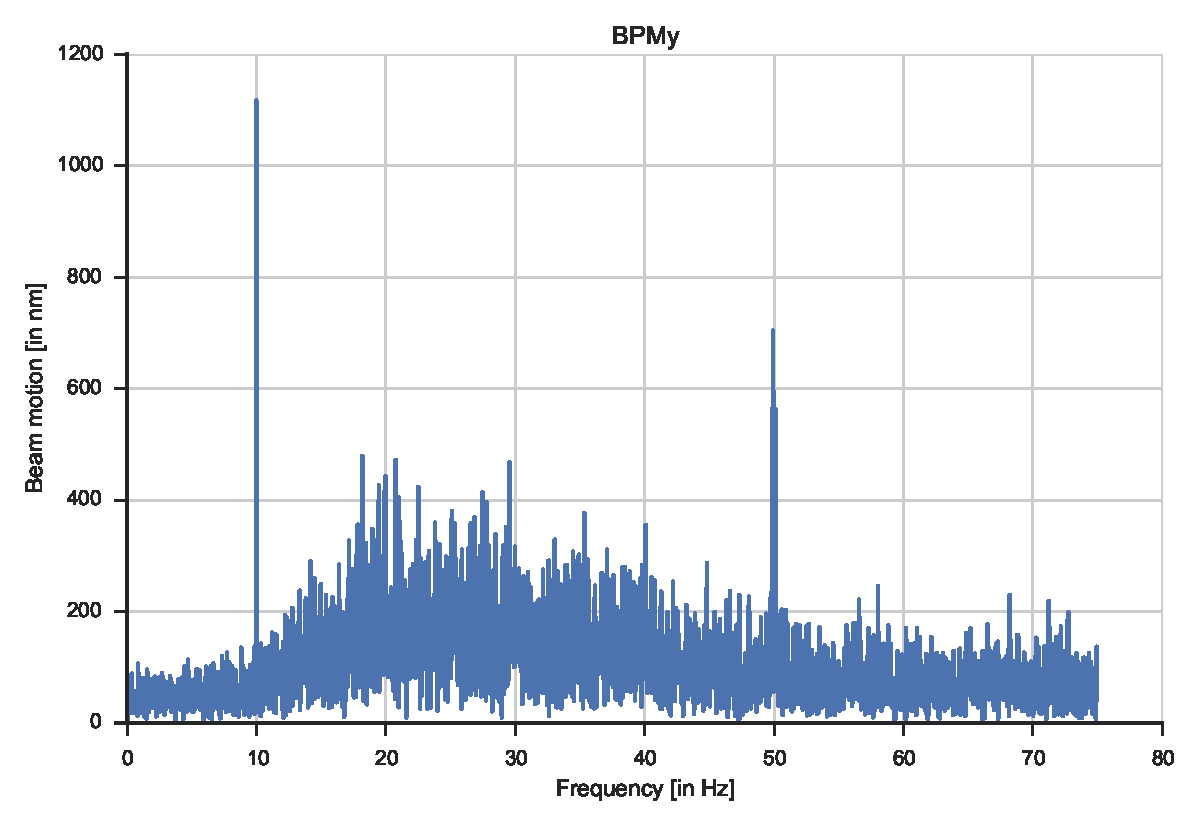
\includegraphics[width=\linewidth]{img/fft_fofb_low}
        \caption{FOFB only}
    \end{subfigure}
%    \hfill
    \begin{subfigure}[b]{0.8\textwidth}
    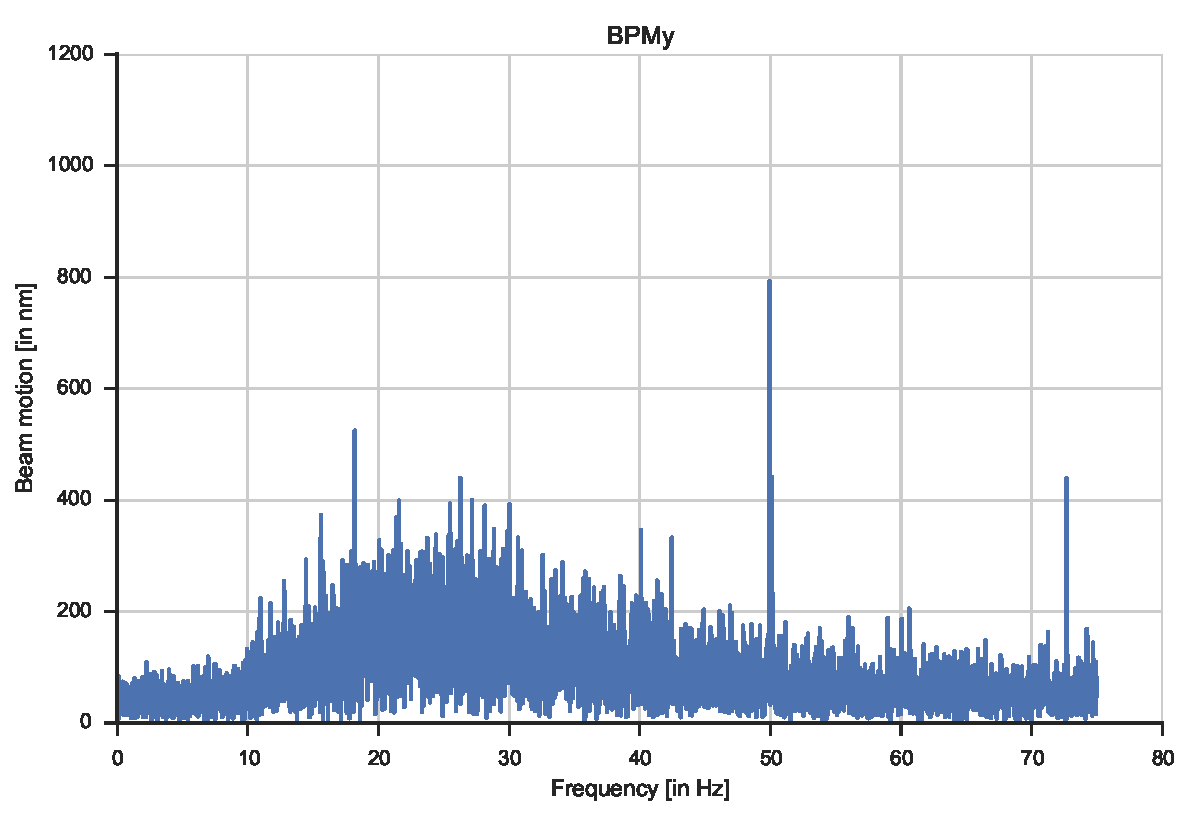
\includegraphics[width=\linewidth]{img/fft_fofb_dyn_low}
    \caption{FOFB + \SI{10}{\hertz} correction}
    \end{subfigure}
    \caption{\label{fig:compare_dyn_corr}Orbit motion spectrum: with and without \SI{10}{\hertz} harmonic correction (vertical, current: \SI{15}{\milli\ampere})}
\end{figure}


\section{System and correction simulation}
One difficulty in improving the current correction process is that machine time is expensive: tests cannot be done very often. A wrong correction can indeed destabilize the orbit or worse, lose the electrons in the vacuum chamber walls, and thus it cannot be tested when the storage ring is on service or other scientists do experiments or measurements for their own research. However, has presented previously, the process is complex and it must be sure that every actors will play correctly in an improved process. Simulating the whole environment is expected to mitigate this.

\subsection{Theoretical background}
\subsubsection{System}
To model a practical process, a system is used. 

A system is defined as an operator $\mathcal{L}$, changing a set of $q$ inputs $\vec{u}$ in into $p$ outputs $\vec{y}$. Generally, the inputs, outputs and operator can vary with time, position, temperature or any possible variable.

For example if the inputs, outputs and operators are only time dependent:
\begin{equation}
	\vec{y}(t) = \mathcal{L}[\vec{u}(t),t]
\end{equation}

\subsubsection{Linear time invariant system}
A linear time invariant (LTI) system is 
\begin{itemize}
	\item \textbf{time invariant}: the operator $\mathcal{L}$ does not depend of the time, meaning that a given input will always generate the same output: $\mathcal{L}[\vec{u},t]=\mathcal{L}[\vec{u}]$. This is can also being described as
	\begin{equation}
		\vec{y}(t) = \mathcal{L}[\vec{u}(t)] \implies \forall \tau, \quad \vec{y}(t-\tau) = \mathcal{L}[\vec{u}(t-\tau)]
	\end{equation}
	\item \textbf{linear}: 	the operator  $\mathcal{L}$ is linear
	\begin{equation}
		\begin{cases}
			\vec{y}_1(t) = \mathcal{L}[\vec{u}_1(t)] \\
			\vec{y}_2(t) = \mathcal{L}[\vec{u}_2(t)] 
		\end{cases}
		\implies \forall (\alpha, \beta) \in \mathbb{R}^2, \quad
		\alpha \vec{y}_1(t) + \beta \vec{y}_2(t) = \mathcal{L}[\alpha\vec{u}_1(t)+\beta\vec{u}_2(t)]
	\end{equation}
	This linearity property allows analyzing any complicated input as a sum of easier ones that will be superposed. The system complexity can thus be more easily handled.
\end{itemize}

It can be proven that in a LTI system, an harmonic input signal of frequency $f_0$ will produced an harmonic output signal with the same frequency. Only the amplitude and the phase will be different.

\subsubsection{Transfer function}
LTI systems can be described with specific operators called transfer functions.

Let a system with a single input and single output (SISO) be described as 
\begin{equation}
	\label{eq:controlth_diff_eq}
	\sum\limits_{k=0}^M a_k \frac{d^k y}{dt^k}(t) = \sum\limits_{j=0}^N b_j \frac{d^j u}{dt^j}(t).
\end{equation}
Taking its Laplace transform yields
\begin{equation}
\sum\limits_{k=0}^N a_k s^k Y(s) = \sum\limits_{j=0}^M b_j s^j U(s).
\end{equation}
where a $Y(s) = \mathcal{L}\{y(t)\}$ and $U(s) = \mathcal{L}\{u(t)\}$ the Laplace transform of its output and input.

The transfer function is defined as
\begin{equation}
	\label{eq:controlth_tf}
	G(s) = \frac{Y(s)}{U(s)} = \frac{\sum\limits_{j=0}^M b_j s^j}{\sum\limits_{k=0}^N a_k s^k}.
\end{equation}

\begin{itemize}
	\item $N$ is the order of the system (i.e. the order of the pole polynomial) 
	\item $N-M$ is the relative order
	\item A system $G(s)$ is defined as \emph{proper} if $\lim\limits_{\omega \rightarrow \infty} G(j\omega) = D \neq \infty$, which requires $M < N$. It means that it can be physically realized.
\end{itemize}

\subsubsection{State-space description}
If transfer functions are a very useful tool (for example to represent the Bode diagram of a function or easily combine successive systems), computing their outputs is not very practical. Another representation is often used, with the help of a inner variable $x(t)$:
\begin{equation}
\begin{cases}
	\dfrac{d \vec{x}}{dt}(t) &= \mat{A}\,\vec{x}(t) + \mat{B}\, \vec{u}(t) \\
	\vec{y}(t) &= \mat{C}\,\vec{x}(t) + \mat{D} \,\vec{u}(t)
\end{cases}
\quad , \qquad \vec{x}(0) = \vec{x}_0
\end{equation}
where $\mat{A} \in \mathbb{R}^{n \times n}$, $\mat{B} \in \mathbb{R}^{n \times q}$, $\mat{C} \in \mathbb{R}^{p \times n}$ and $\mat{D} \in \mathbb{R}^{p \times q}$ can be defined from the transfer function \cref{eq:controlth_tf} or directly from the differential equation model \cref{eq:controlth_tf}. This will not be described here, as Python and \textsc{Matlab} libraries provide functions to directly calculate the matrices. A more thorough reference can be found in \cite{lect:king-ident}.

This representation is however a continuous representation, that cannot be used directly on a DSP. It must be first be transformed as follow \cite{lect:king-ident}, for a sampling rate $F_s = \frac{1}{T_s}$ 
\begin{equation}
	\mat{\tilde{A}} = e^{\mat{A} T_s}, \quad
	\mat{\tilde{B}} = \int_0^{T_s} e^{\mat{A} (T_s-\tau)} \mat{B} d\tau,\quad
	\mat{\tilde{C}} = \mat{C}, \quad
	\mat{\tilde{D}} = \mat{D}
\end{equation}
and then 
\begin{equation}
\label{eq:controlth_ss}
	\begin{cases}
		\vec{x}[k+1] &= \mat{\tilde{A}}\,\vec{x}[k] + \mat{\tilde{B}}\, \vec{u}[k] \\
		\vec{y}[k] &= \mat{\tilde{C}}\,\vec{x}[k] + \mat{\tilde{D}} \,\vec{u}[k]
	\end{cases}
	\quad , \qquad \vec{x}[0] = \vec{x}_0.
\end{equation}

\Cref{eq:controlth_ss} is mostly used in the simulation algorithm.

\subsubsection{Empirical transfer function estimation}
In some cases, modeling the system with differential equation is either to complex or provides to simplistic results. The system can instead being used as a black box, and it's frequency response measured.

\paragraph{Using Fourier transform}
The Laplace transform evaluated in $s=j\omega$ results in the Fourier transform. Therefore, as shown in \cref{eq:controlth_tf}, using an input with enough frequency content should allow getting a good estimation of the transfer function:
\begin{equation}
	\tilde{G}(j\omega) = \frac{Y(j\omega)}{U(j\omega)}.
\end{equation}
However this naive method is not really used in practice as the measurement noises and artifacts in the output would have strong impact on the estimation.

\paragraph{Spectral density}
A better method is to use the spectral density and the cross-spectral density.

In the time domain, the output can be written as a function of the input by using a impulse response $g(t) = \mathcal{L}^{-1}\{G(s)\}$
\begin{equation}
	y(t) = g * u\,(t) =  \int_0^{+\infty} g(\tau) u(t-\tau)d\tau
\end{equation}

The cross-correlation between the input and the output is given by
\begin{align}
R_{uy}(\tau) &= E \left\{ u(t) y(t+\tau)\right\} \nonumber\\
			 &= E \left\{ u(t) \int_0^{+\infty} g(v) u(t+\tau-v)dv\right\} \nonumber\\
			 &= ... \nonumber \\ 
			 &= \int_0^{+\infty} g(v) R_{uu}(\tau-v) dv \nonumber\\
			 &= g * R_{uu} \, (\tau)
\end{align}
where $R_{uu}$ is the autocorrelation of the input. Transforming this equation to the frequency domain yields
\begin{equation}
	S_{uy}(j\omega) = G(j\omega)\cdot S_{uu}(j\omega)   \iff 	G(j\omega) = \frac{S_{uy}(j\omega) }{ S_{uu}(j\omega)}
\end{equation}
where $S_{uy}$ is the cross-spectral density and $S_{uu}$ the spectral density of the input.

This provides better results in practice because only the relevant information of the signal is used: the transfer function estimation is less dependent of the measurement noise and other possible artifacts.

\paragraph{Correct input}
It is important to choose a good input signal. It must contain enough harmonic components to provide an estimation of the full spectrum. Literature often propose a pink noise or a sine-sweep.

A pink noise is a signal which power spectrum is decreasing like $1/\omega$. The spectrum is thus fully represented, with high frequencies having less impact and therefore being less likely to harm the system. In a system like the storage ring, using a noise as input is however not a good idea. 

A sine sweep is a sine which frequency increases with the time, so that every frequencies are represented. A linear increase can be obtained by setting
\begin{equation}
	f(t) = 2 f_\text{min} \cdot t + \frac{f_\text{max}-f_\text{min}}{2 \cdot t_\text{max}} t^2
\end{equation}
The input is then
\begin{equation}
	u(t) = A \sin(2\pi f(t))
\end{equation}

\subsection{System identification}
The first step in the model is to represent the storage ring. This could be done analytically, by writing the magnet equations and deriving the full differential equations that bind the correction to orbit displacement. However, it would take a full master thesis to realize a good model, as there are very different types of components all around the orbit, with some non-linear, some coupled and complex behaviors.

Instead a system identification is conducted. The system is the storage ring, with the differential orbit as the output, and correction magnet amplitude as input. It is assumed that the system can be modeled as a first approximation as a SISO system, generalized as a MIMO one by pre-multiplying it by the response matrix (which is a mere gain):
\begin{equation}
	\Delta \vec{X}(t) = \mat{S}\cdot \left[ g * \Delta\vec{\theta} \, (t) \right]
\end{equation}

A sine sweep was designed to cover from $f_\text{min} = 0$ to $f_\text{max} = F_s/2 = \SI{75}{\hertz}$ and used as the corrector magnets input (one by one).

By using the (cross-)spectral density of the input and output signal, an experimental estimation of the transfer function is provided. The estimation is then fitted with a \textsc{Matlab} routine implementing the Fast Relaxed Vector Fitting \cite{art:vfit3-1, art:vfit3-2, art:vfit3-3, web:vfit3} and provides the continuous time state-space matrices $\mat{A}$, $\mat{B}$, $\mat{C}$ and $\mat{D}$. The result is shown \cref{fig:ctl_vfit3}.

\begin{figure}
	\begin{subfigure}[t]{0.5\linewidth}
		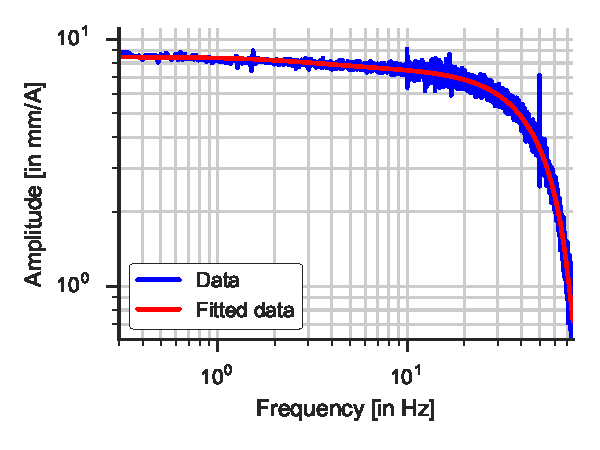
\includegraphics[width=1\linewidth]{img/ctl_id_amplitude}
		\caption{Amplitude}
	\end{subfigure}
	\hfill
	\begin{subfigure}[t]{0.5\linewidth}
		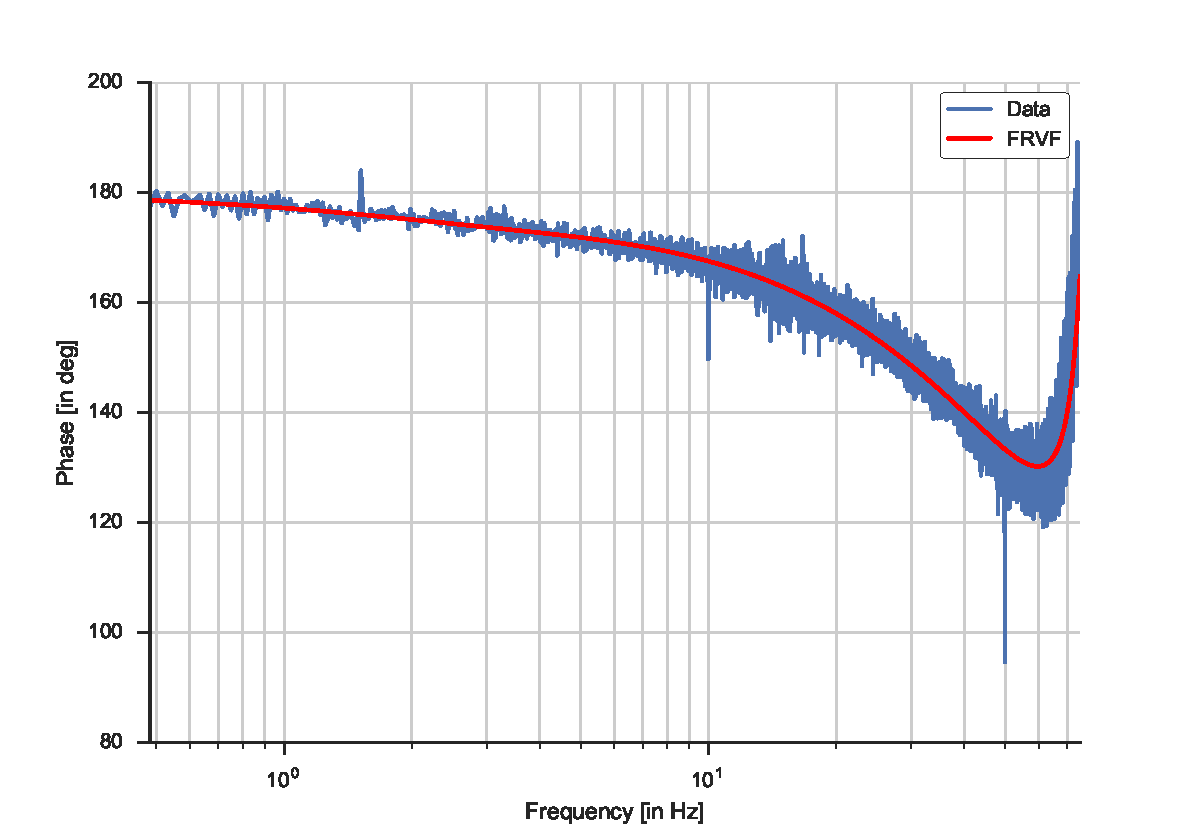
\includegraphics[width=1\linewidth]{img/ctl_id_phase}
		\caption{Phase}
	\end{subfigure}
	\caption{\label{fig:ctl_vfit3}Results of the vector fitting with vfit3}
\end{figure}

It appeared that after converting the system to a transfer function, the numerator was complex. Taking only the real part of each coefficient provided a solution that still fitted the experimental data. In order to obtain a transfer function usable with the response matrix, it was normalized so that its ground gain was 1.

\Cref{fig:ctl_vfit3} shows however only the frequency domain below \SI{75}{\hertz}. In the first simulations, it appeared that the step response presented a large spike which was hardly physically possible (see \cref{fig:ctl_id_spike}). To correct this, the numerator highest degree coefficient was set to 0, which led to the result given in \cref{fig:ctl_id_nospike}. 

\begin{figure}
	\begin{subfigure}[t]{0.5\linewidth}
		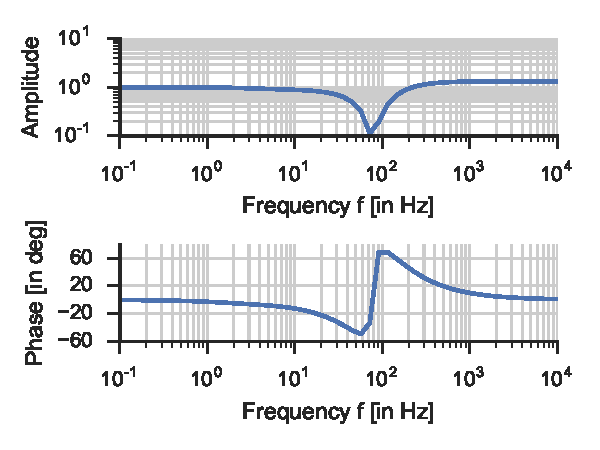
\includegraphics[width=1\linewidth]{img/ctl_id_3z}
		\caption{Frequency response}
	\end{subfigure}
	\hfill
	\begin{subfigure}[t]{0.5\linewidth}
		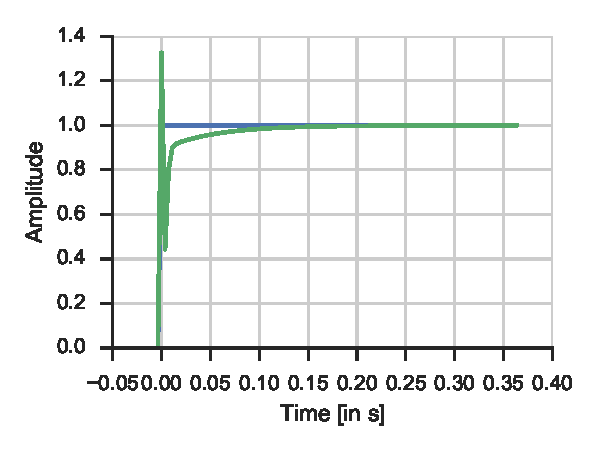
\includegraphics[width=1\linewidth]{img/ctl_id_3z_step}
		\caption{Step response}
	\end{subfigure}
	\caption{\label{fig:ctl_id_spike}Normalized transfer function}
\end{figure}

\begin{figure}
	\begin{subfigure}[t]{0.5\linewidth}
		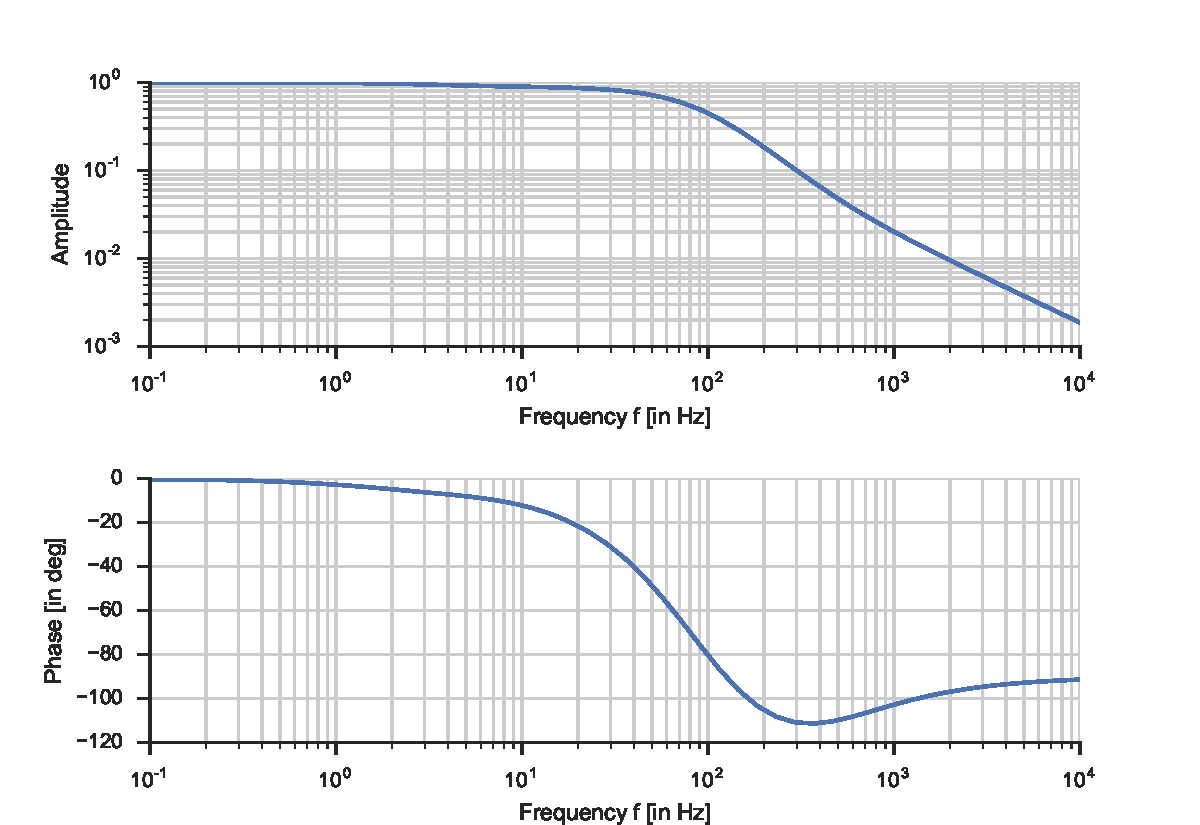
\includegraphics[width=1\linewidth]{img/ctl_id_2z}
		\caption{Frequency response}
	\end{subfigure}
	\hfill
	\begin{subfigure}[t]{0.5\linewidth}
		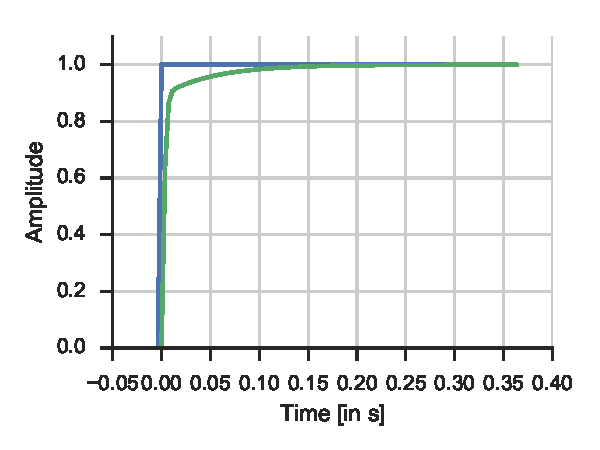
\includegraphics[width=1\linewidth]{img/ctl_id_2z_step}
		\caption{Step response}
	\end{subfigure}
	\caption{\label{fig:ctl_id_nospike}Normalized, zeros-corrected transfer function}
\end{figure}

Finally it the transfer function estimation is 
\begin{equation}
G(s) = \frac{117.322203 \,s^2 + 319144.577 \,s + 6801819.36}
{s^3 + 1171.05630 \,s^2 + 375569.975 \,s +	6801819.36}
\end{equation}

The frequency response given in \cref{fig:ctl_id_nospike} corresponds to what was expected: an amplitude that decreases with frequencies, without amplification domain. To be sure that it corresponds to reality, a simulation of the current situation was conducted.

\subsection{Simulation model}
\label{sec:correction_simulation}

In order to represent at best the environment, the simulation needs to take in account computation delays and that the correction happens at a given sampled time \SI{150}{\hertz}) whereas other systems perform in continuous time. To achieve that, the simulation is played step by step, at \SI{150}{\hertz} for the correction process and \SI{1.5}{\kilo\hertz} for the continuous time.

\Cref{fig:model_simul} represents the block diagram of the environment, $\text{H}_\text{ring}$ being the identified transfer function of storage ring, and the low pass filter representing the averaging of orbit values in the BPM recording. A initial correction $\vec{\theta}_0$, which is normally provided by a punctual correction process (the slow orbit feedback or SOFB), is needed to ensure the stability of the orbit.

\begin{sidewaysfigure}
    \centering
    \begin{tikzpicture}[auto, node distance=1,>=latex']
%    \draw[help lines, yellow] (-1,-4)grid(15,3);
    \draw [dashed, black] (-.5, 1.7) -- (10.1, 1.7) -- (10.1, -3.5) -- (-.5, -3.5) -- cycle;
    \draw [black](2.8, -3.7) node [above right=0 0.2] {\small mBox --- $F_s=\SI{150}{\hertz}$};

    % We start by placing the blocks
    \node [input] (xref) {};
    \node [operator, right=1.5 of xref] (sum) {$+$};
    \node [operator, right=of sum] (xsmat) {$\times$};
    \node [input, above=of xsmat] (smat) {};
    \node [block, right=of xsmat] (corrector) {K};
    \node [operator, right=of corrector] (suminit) {+};
    \node [input, above=of suminit] (initval) {};
    \node [block, right=of suminit] (DAC) {$\uparrow$};
    \node [block, right=of DAC] (delay) {$\begin{matrix}\text{Delay T}\\\text{\footnotesize Computation}\end{matrix}$};
    \node [operator, right=of delay] (sumperturb) {$+$};
    \node [input, above=of sumperturb] (perturb) {};
    \node [block, right=of sumperturb] (Hring) {$\text{H}_\text{ring}$};
    \node [block, below=of delay] (lowpass) {Low pass};
    \node [block, below=of DAC] (ADC) {$\downarrow$ \SI{150}{\hertz}};
    \coordinate [right= of Hring] (connectout) {};
    \node [input, right= of connectout] (out) {};
    
    % Once the nodes are placed, connecting them is easy.
    \draw [->] (xref)     	-- node [pos=0.2] {$\vec{X}_\text{ref}$} (sum);
    \draw [->] (sum)      	-- node {$\Delta\vec{X}$}    	(xsmat);
    \draw [->] (smat)      	-- node {$\mat{S}*$}    	    (xsmat);
    \draw [->] (xsmat)  	-- node {}                   	(corrector);
    \draw [->] (corrector) 	-- node {$\Delta\vec{\Theta}$} 	(suminit);
    \draw [->] (initval) 	-- node {$\vec{\Theta}_0$}      (suminit);
    \draw [->] (suminit)  	-- node {$\vec{\Theta}$}        (DAC);
    \draw [->] (DAC)      	-- node {}                   	(delay);
    \draw [->] (delay)    	-- node {$\theta(t)$}         	(sumperturb);
    \draw [->] (perturb)  	-- node {$d(t)$}               	(sumperturb);
    \draw [->] (sumperturb) -- node {}                		(Hring);
    \draw [-]  (Hring)    	-- node {}                 		(connectout);
    \draw [->] (connectout) -- node {$x(t)$}          		(out);
    \draw [->] (connectout) |- node {}                 		(lowpass);
    \draw [->] (lowpass)    -- node {}                 		(ADC);
	\draw [->] (ADC)     	-| node[pos=0.5] {$\vec{X}$}
                               node [pos=0.90, left]{$-$}	(sum.south);
    \end{tikzpicture}
    \caption{\label{fig:model_simul}The full model, K being the corrector to define}
\end{sidewaysfigure}

\subsection{Simulation results}
Several scenari were designed to validate the simulation, and propose some enhancement to current correction. The delay of the computation is approximated by $\delta t = \SI{3}{\milli\second}$.
 
\subsubsection{Current configuration at BESSY~II}
To represent the current configuration in BESSY~II, the PID corrector presented in \cref{sec:correction_state_of_art} was implemented as a pure integrator of amplitude 0.8. The closed-loop system frequency response would be as given in \cref{fig:ctl_freqresp_pid}. As in the reality, frequencies below \SI{10}{\hertz} are damped, and are slightly amplified above. Applying the simulation step by step with a plausible perturbation leads to the result presented in \cref{fig:ctl_sim_pid}.

\begin{figure}
    \centering
    \begin{subfigure}{0.49\textwidth}
        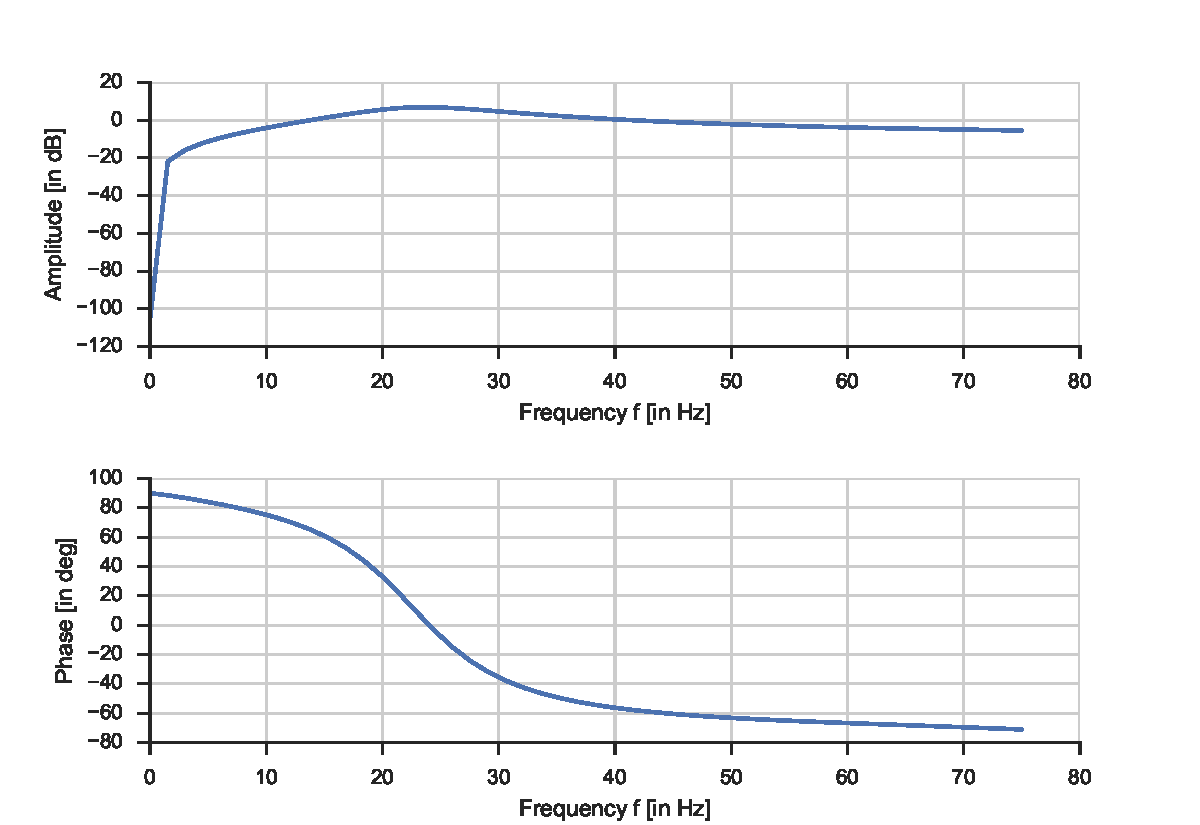
\includegraphics[width=\textwidth]{img/ctl_freqresp_pid}
        \caption{\label{fig:ctl_freqresp_pid} Bode diagram of the closed-loop}
    \end{subfigure}
    \hfill
    \begin{subfigure}{0.49\textwidth}
        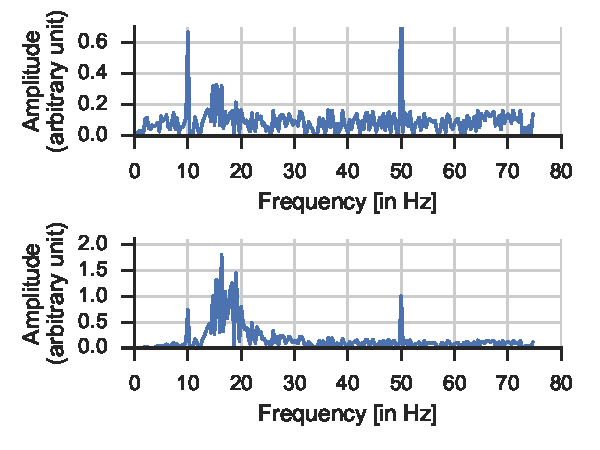
\includegraphics[width=\textwidth]{img/ctl_sim_pid}
        \caption{\label{fig:ctl_sim_pid}Simulation}
        \end{subfigure}    
    \caption{Frequency response for K = PID(0, $0.8\cdot F_s$, 0)}
\end{figure}

The PID can then be slightly enhanced by finding better coefficients, for example with K~=~PID($0.9$, $0.5\cdot F_s$, $0.15/F_s$), which result can be seen in \cref{fig:ctl_freqresp_bestpid,fig:ctl_sim_bestpid}. It can be seen there that more frequencies are slightly damped and that the amplified area is smaller, with less gain, providing better results.

\begin{figure}
    \centering
    \begin{subfigure}{0.49\textwidth}
        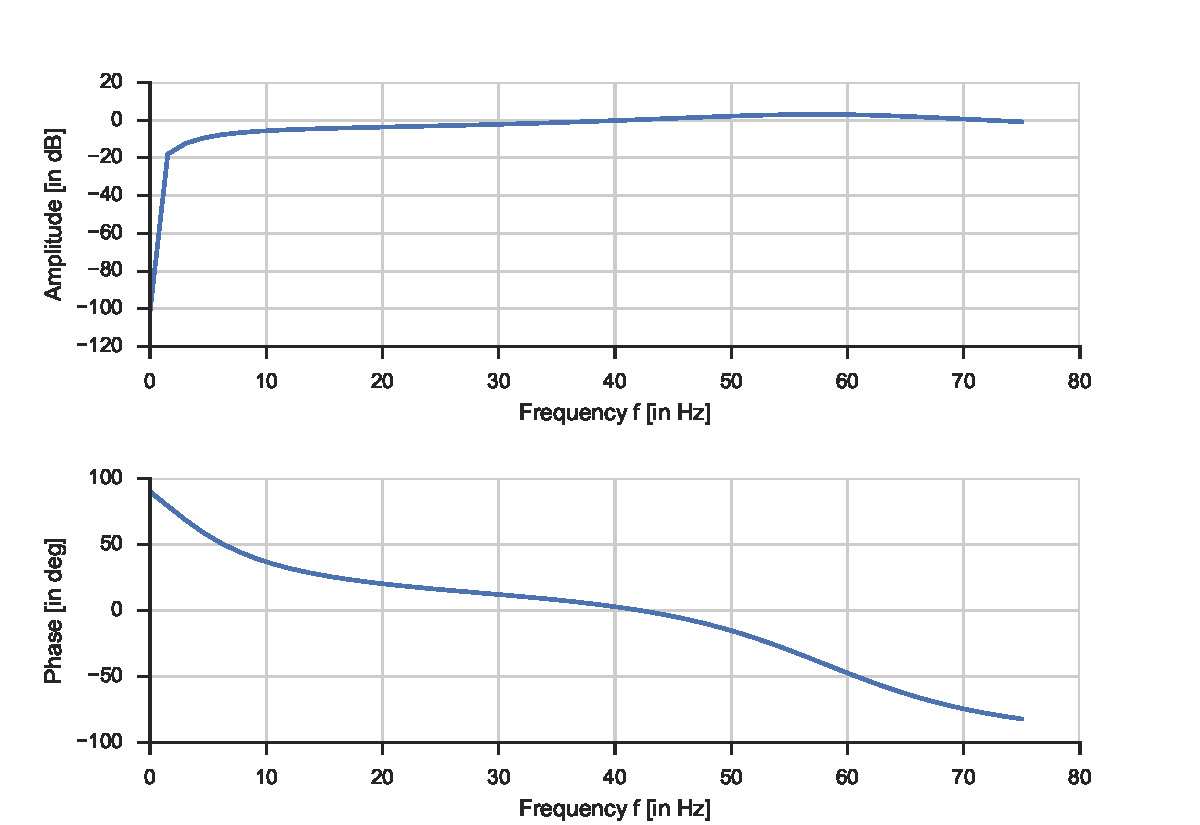
\includegraphics[width=\textwidth]{img/ctl_freqresp_bestpid}
        \caption{\label{fig:ctl_freqresp_bestpid} Bode diagram of the closed-loop}
    \end{subfigure}
    \hfill
    \begin{subfigure}{0.49\textwidth}
        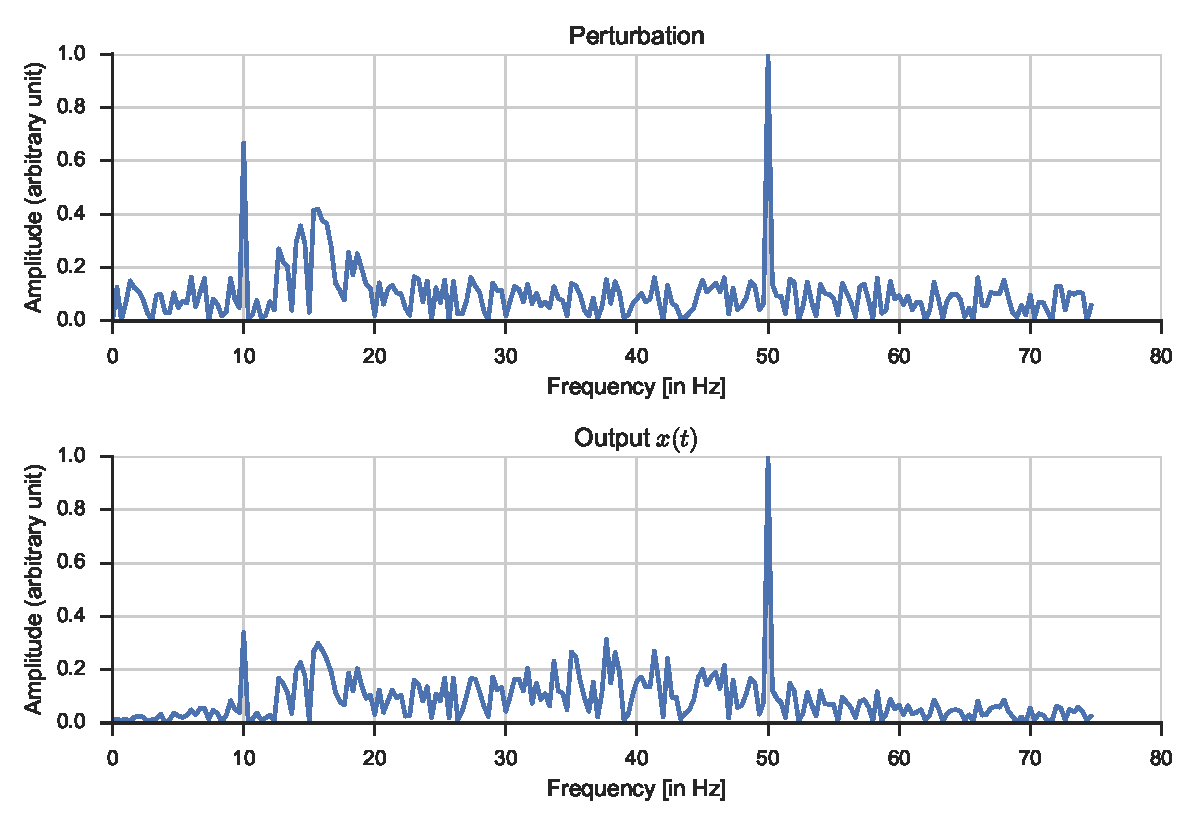
\includegraphics[width=\textwidth]{img/ctl_sim_bestpid}
        \caption{\label{fig:ctl_sim_bestpid}Simulation}
    \end{subfigure}    
    \caption{Frequency response for a better PID}
\end{figure}

\subsubsection{Optimal correction}
Following the design rules defined in \cite{book:Skogestad-2005}, one can synthesize an $\mathcal{H}_\infty$-corrector, which is an optimal corrector obtained by optimizing the closed and opened loop over the $\infty$-norm\footnote{The $\infty$-norm is defined for vectors as $||\vec{x}||_\infty = \max\limits_{i} |x_i|$} with given parameters. The Robust Control Toolbox from \textsc{Matlab} was used for this effect. The \textsc{Matlab} script given below is an adapted copy of what can be found in Skogestad \cite{book:Skogestad-2005}, page 60. The computation delay is modeled with the Padé approximation of first order \cite{book:matrix} provided by \textsc{Matlab} and added to the system, so that the corrector takes this in account.
\begin{Matlab}
% The robust control toolbox is needed.

% Load ring transfert function
[G_num, G_den] = load(G) 

% Create delay
delay = 0.003;
[dnum, dden] = pade(delay, 1);

G = nd2sys(conv(G_num,d_num),conv(G_den,d_den),1);

% Define parameters
fb = 30  % Bandwidth
wb = fb*2*pi;  
M = 1.001;  % Lim sup (high freq.)
Am = 10^-4;  % Lim sup (low freq.)

% Create weights
Wp = nd2sys([1/M wb], [1 wb*Am]);
Wu = 1;

% Define the system
systemnames = 'G Wp Wu';
inputvar = '[r(1) ; u(1)]';
outputvar = '[Wp; Wu; r-G]';
input_to_G = '[u]';
input_to_Wp = '[r-G]';
input_to_Wu = '[u]';
sysoutname = 'P';
cleanupsysic = 'yes';
sysic;

% Compute corrector
nmeas=1; nu=1; gmn=0.5; gmx=20; tol=0.001;
[khinf,ghinf,gopt] = hinfsyn(P,nmeas,nu,gmn,gmx,tol);
\end{Matlab}

This provides a corrector, which frequency response can be seen in \cref{fig:ctl_freqresp_hinf}: very efficient in low frequencies, it has however an amplification area that can be a problem. Correctors with different bandwidth where synthesize. The simulation is given in \cref{fig:ctl_sim_hinf}. The results are strangely enough always less efficient than the proposed PID (in \cref{fig:ctl_freqresp_bestpid}). \todo{$\mathcal{H}_\infty$: Review this part with Maxim}

\begin{figure}
    \centering
    \begin{subfigure}{0.49\textwidth}
        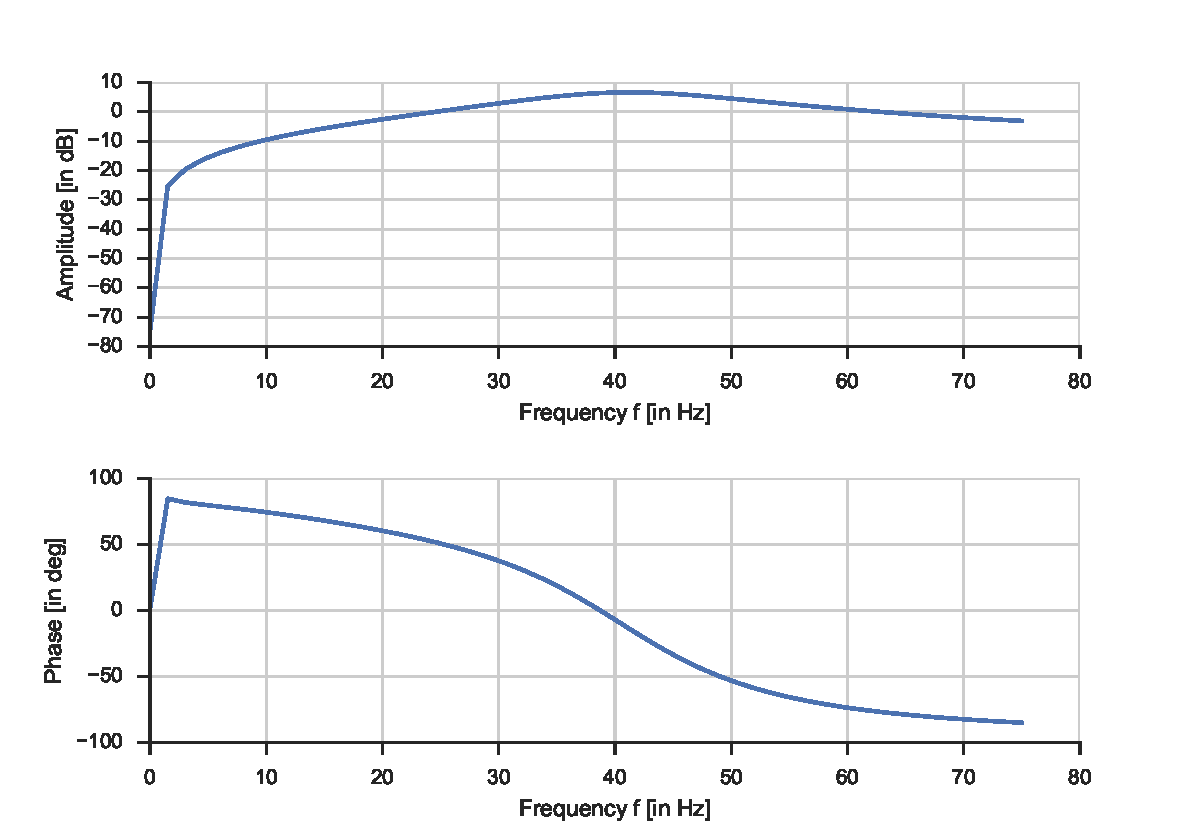
\includegraphics[width=\textwidth]{img/ctl_freqresp_hinf}
        \caption{\label{fig:ctl_freqresp_hinf} Bode diagram of the closed-loop, $f_b$ = \SI{50}{Hz}}
    \end{subfigure}
    \hfill
    \begin{subfigure}{0.49\textwidth}
        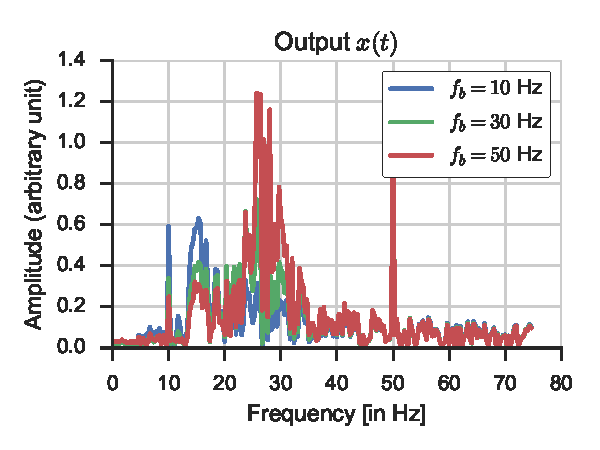
\includegraphics[width=\textwidth]{img/ctl_sim_hinf}
        \caption{\label{fig:ctl_sim_hinf}Simulation (several bandwidths)}
    \end{subfigure}    
    \caption{Frequency response of $\mathcal{H}_\infty$-correctors}
\end{figure}

\section{Summary}
In order to be sure that the electron beam remains focused and stable, a control process is needed. The concerned hardware and software stack at BESSY~II was first studied and the main actor (the mBox) modernized. To the original correction was added a dynamic correction, that can correct static harmonic perturbations and have them almost completely disappear.

In parallel, a simulation environment was built in order to be able to predict the influence of some parameters on the system and to closely study how to correct at best the orbit position. From this was predicted that a more optimized PID corrector is possible, which only needs to be validated experimentally. The optimal correction direction must be considered in more depth and, on a more ambitious perspective, the design of robust MIMO correctors would certainly provide better and more reliable results.